\documentclass[1p]{elsarticle_modified}
%\bibliographystyle{elsarticle-num}

%\usepackage[colorlinks]{hyperref}
%\usepackage{abbrmath_seonhwa} %\Abb, \Ascr, \Acal ,\Abf, \Afrak
\usepackage{amsfonts}
\usepackage{amssymb}
\usepackage{amsmath}
\usepackage{amsthm}
\usepackage{scalefnt}
\usepackage{amsbsy}
\usepackage{kotex}
\usepackage{caption}
\usepackage{subfig}
\usepackage{color}
\usepackage{graphicx}
\usepackage{xcolor} %% white, black, red, green, blue, cyan, magenta, yellow
\usepackage{float}
\usepackage{setspace}
\usepackage{hyperref}

\usepackage{tikz}
\usetikzlibrary{arrows}

\usepackage{multirow}
\usepackage{array} % fixed length table
\usepackage{hhline}

%%%%%%%%%%%%%%%%%%%%%
\makeatletter
\renewcommand*\env@matrix[1][\arraystretch]{%
	\edef\arraystretch{#1}%
	\hskip -\arraycolsep
	\let\@ifnextchar\new@ifnextchar
	\array{*\c@MaxMatrixCols c}}
\makeatother %https://tex.stackexchange.com/questions/14071/how-can-i-increase-the-line-spacing-in-a-matrix
%%%%%%%%%%%%%%%

\usepackage[normalem]{ulem}

\newcommand{\msout}[1]{\ifmmode\text{\sout{\ensuremath{#1}}}\else\sout{#1}\fi}
%SOURCE: \msout is \stkout macro in https://tex.stackexchange.com/questions/20609/strikeout-in-math-mode

\newcommand{\cancel}[1]{
	\ifmmode
	{\color{red}\msout{#1}}
	\else
	{\color{red}\sout{#1}}
	\fi
}

\newcommand{\add}[1]{
	{\color{blue}\uwave{#1}}
}

\newcommand{\replace}[2]{
	\ifmmode
	{\color{red}\msout{#1}}{\color{blue}\uwave{#2}}
	\else
	{\color{red}\sout{#1}}{\color{blue}\uwave{#2}}
	\fi
}

\newcommand{\Sol}{\mathcal{S}} %segment
\newcommand{\D}{D} %diagram
\newcommand{\A}{\mathcal{A}} %arc


%%%%%%%%%%%%%%%%%%%%%%%%%%%%%5 test

\def\sl{\operatorname{\textup{SL}}(2,\Cbb)}
\def\psl{\operatorname{\textup{PSL}}(2,\Cbb)}
\def\quan{\mkern 1mu \triangleright \mkern 1mu}

\theoremstyle{definition}
\newtheorem{thm}{Theorem}[section]
\newtheorem{prop}[thm]{Proposition}
\newtheorem{lem}[thm]{Lemma}
\newtheorem{ques}[thm]{Question}
\newtheorem{cor}[thm]{Corollary}
\newtheorem{defn}[thm]{Definition}
\newtheorem{exam}[thm]{Example}
\newtheorem{rmk}[thm]{Remark}
\newtheorem{alg}[thm]{Algorithm}

\newcommand{\I}{\sqrt{-1}}
\begin{document}

%\begin{frontmatter}
%
%\title{Boundary parabolic representations of knots up to 8 crossings}
%
%%% Group authors per affiliation:
%\author{Yunhi Cho} 
%\address{Department of Mathematics, University of Seoul, Seoul, Korea}
%\ead{yhcho@uos.ac.kr}
%
%
%\author{Seonhwa Kim} %\fnref{s_kim}}
%\address{Center for Geometry and Physics, Institute for Basic Science, Pohang, 37673, Korea}
%\ead{ryeona17@ibs.re.kr}
%
%\author{Hyuk Kim}
%\address{Department of Mathematical Sciences, Seoul National University, Seoul 08826, Korea}
%\ead{hyukkim@snu.ac.kr}
%
%\author{Seokbeom Yoon}
%\address{Department of Mathematical Sciences, Seoul National University, Seoul, 08826,  Korea}
%\ead{sbyoon15@snu.ac.kr}
%
%\begin{abstract}
%We find all boundary parabolic representation of knots up to 8 crossings.
%
%\end{abstract}
%\begin{keyword}
%    \MSC[2010] 57M25 
%\end{keyword}
%
%\end{frontmatter}

%\linenumbers
%\tableofcontents
%
\newcommand\colored[1]{\textcolor{white}{\rule[-0.35ex]{0.8em}{1.4ex}}\kern-0.8em\color{red} #1}%
%\newcommand\colored[1]{\textcolor{white}{ #1}\kern-2.17ex	\textcolor{white}{ #1}\kern-1.81ex	\textcolor{white}{ #1}\kern-2.15ex\color{red}#1	}

{\Large $\underline{12a_{0151}~(K12a_{0151})}$}

\setlength{\tabcolsep}{10pt}
\renewcommand{\arraystretch}{1.6}
\vspace{1cm}\begin{tabular}{m{100pt}>{\centering\arraybackslash}m{274pt}}
\multirow{5}{120pt}{
	\centering
	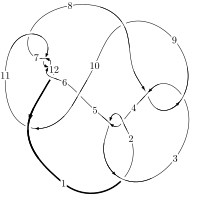
\includegraphics[width=112pt]{../../../GIT/diagram.site/Diagrams/png/952_12a_0151.png}\\
\ \ \ A knot diagram\footnotemark}&
\allowdisplaybreaks
\textbf{Linearized knot diagam} \\
\cline{2-2}
 &
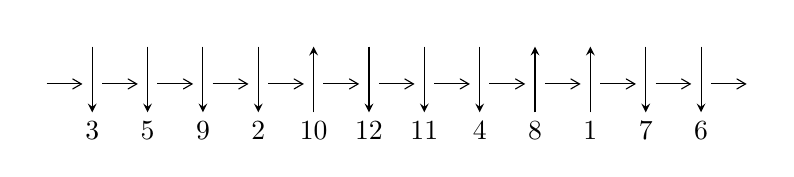
\begin{tikzpicture}[x=20pt, y=17pt]
	% nodes
	\node (C0) at (0, 0) {};
	\node (C1) at (1, 0) {};
	\node (C1U) at (1, +1) {};
	\node (C1D) at (1, -1) {3};

	\node (C2) at (2, 0) {};
	\node (C2U) at (2, +1) {};
	\node (C2D) at (2, -1) {5};

	\node (C3) at (3, 0) {};
	\node (C3U) at (3, +1) {};
	\node (C3D) at (3, -1) {9};

	\node (C4) at (4, 0) {};
	\node (C4U) at (4, +1) {};
	\node (C4D) at (4, -1) {2};

	\node (C5) at (5, 0) {};
	\node (C5U) at (5, +1) {};
	\node (C5D) at (5, -1) {10};

	\node (C6) at (6, 0) {};
	\node (C6U) at (6, +1) {};
	\node (C6D) at (6, -1) {12};

	\node (C7) at (7, 0) {};
	\node (C7U) at (7, +1) {};
	\node (C7D) at (7, -1) {11};

	\node (C8) at (8, 0) {};
	\node (C8U) at (8, +1) {};
	\node (C8D) at (8, -1) {4};

	\node (C9) at (9, 0) {};
	\node (C9U) at (9, +1) {};
	\node (C9D) at (9, -1) {8};

	\node (C10) at (10, 0) {};
	\node (C10U) at (10, +1) {};
	\node (C10D) at (10, -1) {1};

	\node (C11) at (11, 0) {};
	\node (C11U) at (11, +1) {};
	\node (C11D) at (11, -1) {7};

	\node (C12) at (12, 0) {};
	\node (C12U) at (12, +1) {};
	\node (C12D) at (12, -1) {6};
	\node (C13) at (13, 0) {};

	% arrows
	\draw[->,>={angle 60}]
	(C0) edge (C1) (C1) edge (C2) (C2) edge (C3) (C3) edge (C4) (C4) edge (C5) (C5) edge (C6) (C6) edge (C7) (C7) edge (C8) (C8) edge (C9) (C9) edge (C10) (C10) edge (C11) (C11) edge (C12) (C12) edge (C13) ;	\draw[->,>=stealth]
	(C1U) edge (C1D) (C2U) edge (C2D) (C3U) edge (C3D) (C4U) edge (C4D) (C5D) edge (C5U) (C6U) edge (C6D) (C7U) edge (C7D) (C8U) edge (C8D) (C9D) edge (C9U) (C10D) edge (C10U) (C11U) edge (C11D) (C12U) edge (C12D) ;
	\end{tikzpicture} \\
\hhline{~~} \\& 
\textbf{Solving Sequence} \\ \cline{2-2} 
 &
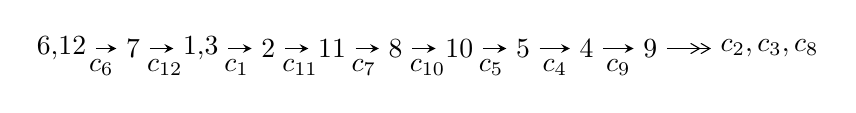
\begin{tikzpicture}[x=23pt, y=7pt]
	% node
	\node (A0) at (-1/8, 0) {6,12};
	\node (A1) at (1, 0) {7};
	\node (A2) at (33/16, 0) {1,3};
	\node (A3) at (25/8, 0) {2};
	\node (A4) at (33/8, 0) {11};
	\node (A5) at (41/8, 0) {8};
	\node (A6) at (49/8, 0) {10};
	\node (A7) at (57/8, 0) {5};
	\node (A8) at (65/8, 0) {4};
	\node (A9) at (73/8, 0) {9};
	\node (C1) at (1/2, -1) {$c_{6}$};
	\node (C2) at (3/2, -1) {$c_{12}$};
	\node (C3) at (21/8, -1) {$c_{1}$};
	\node (C4) at (29/8, -1) {$c_{11}$};
	\node (C5) at (37/8, -1) {$c_{7}$};
	\node (C6) at (45/8, -1) {$c_{10}$};
	\node (C7) at (53/8, -1) {$c_{5}$};
	\node (C8) at (61/8, -1) {$c_{4}$};
	\node (C9) at (69/8, -1) {$c_{9}$};
	\node (A10) at (11, 0) {$c_{2},c_{3},c_{8}$};

	% edge
	\draw[->,>=stealth]	
	(A0) edge (A1) (A1) edge (A2) (A2) edge (A3) (A3) edge (A4) (A4) edge (A5) (A5) edge (A6) (A6) edge (A7) (A7) edge (A8) (A8) edge (A9) ;
	\draw[->>,>={angle 60}]	
	(A9) edge (A10);
\end{tikzpicture} \\ 

\end{tabular} \\

\footnotetext{
The image of knot diagram is generated by the software ``\textbf{Draw programme}" developed by Andrew Bartholomew(\url{http://www.layer8.co.uk/maths/draw/index.htm\#Running-draw}), where we modified some parts for our purpose(\url{https://github.com/CATsTAILs/LinksPainter}).
}\phantom \\ \newline 
\centering \textbf{Ideals for irreducible components\footnotemark of $X_{\text{par}}$} 
 
\begin{align*}
I^u_{1}&=\langle 
u^{74}+41 u^{72}+\cdots+b+1,\;- u^{76}+2 u^{75}+\cdots+a- u,\;u^{77}-2 u^{76}+\cdots- u+1\rangle \\
I^u_{2}&=\langle 
b+1,\;- u^3+u^2+a-3 u+1,\;u^4- u^3+3 u^2-2 u+1\rangle \\
\\
\end{align*}
\raggedright * 2 irreducible components of $\dim_{\mathbb{C}}=0$, with total 81 representations.\\
\footnotetext{All coefficients of polynomials are rational numbers. But the coefficients are sometimes approximated in decimal forms when there is not enough margin.}
\newpage
\renewcommand{\arraystretch}{1}
\centering \section*{I. $I^u_{1}= \langle u^{74}+41 u^{72}+\cdots+b+1,\;- u^{76}+2 u^{75}+\cdots+a- u,\;u^{77}-2 u^{76}+\cdots- u+1 \rangle$}
\flushleft \textbf{(i) Arc colorings}\\
\begin{tabular}{m{7pt} m{180pt} m{7pt} m{180pt} }
\flushright $a_{6}=$&$\begin{pmatrix}1\\0\end{pmatrix}$ \\
\flushright $a_{12}=$&$\begin{pmatrix}0\\u\end{pmatrix}$ \\
\flushright $a_{7}=$&$\begin{pmatrix}1\\u^2\end{pmatrix}$ \\
\flushright $a_{1}=$&$\begin{pmatrix}- u\\u\end{pmatrix}$ \\
\flushright $a_{3}=$&$\begin{pmatrix}u^{76}-2 u^{75}+\cdots+5 u^2+u\\- u^{74}-41 u^{72}+\cdots+3 u^2-1\end{pmatrix}$ \\
\flushright $a_{2}=$&$\begin{pmatrix}u^{76}-2 u^{75}+\cdots+5 u^2+2 u\\- u^{73}+u^{72}+\cdots+u-1\end{pmatrix}$ \\
\flushright $a_{11}=$&$\begin{pmatrix}u\\u^3+u\end{pmatrix}$ \\
\flushright $a_{8}=$&$\begin{pmatrix}u^2+1\\u^4+2 u^2\end{pmatrix}$ \\
\flushright $a_{10}=$&$\begin{pmatrix}- u^5-2 u^3+u\\u^5+3 u^3+u\end{pmatrix}$ \\
\flushright $a_{5}=$&$\begin{pmatrix}- u^{10}-5 u^8-6 u^6+u^4+u^2+1\\u^{10}+6 u^8+11 u^6+6 u^4+u^2\end{pmatrix}$ \\
\flushright $a_{4}=$&$\begin{pmatrix}u^{76}-2 u^{75}+\cdots+2 u+1\\u^{74}-2 u^{73}+\cdots+u-1\end{pmatrix}$ \\
\flushright $a_{9}=$&$\begin{pmatrix}- u^{11}-6 u^9-12 u^7-10 u^5-5 u^3\\- u^{13}-7 u^{11}-17 u^9-16 u^7-4 u^5+u^3+u\end{pmatrix}$\\&\end{tabular}
\flushleft \textbf{(ii) Obstruction class $= -1$}\\~\\
\flushleft \textbf{(iii) Cusp Shapes $= - u^{76}+2 u^{75}+\cdots+2 u-5$}\\~\\
\newpage\renewcommand{\arraystretch}{1}
\flushleft \textbf{(iv) u-Polynomials at the component}\newline \\
\begin{tabular}{m{50pt}|m{274pt}}
Crossings & \hspace{64pt}u-Polynomials at each crossing \\
\hline $$\begin{aligned}c_{1}\end{aligned}$$&$\begin{aligned}
&u^{77}+41 u^{76}+\cdots+5 u+1
\end{aligned}$\\
\hline $$\begin{aligned}c_{2},c_{4}\end{aligned}$$&$\begin{aligned}
&u^{77}-5 u^{76}+\cdots-5 u+1
\end{aligned}$\\
\hline $$\begin{aligned}c_{3},c_{8}\end{aligned}$$&$\begin{aligned}
&u^{77}- u^{76}+\cdots+8 u+16
\end{aligned}$\\
\hline $$\begin{aligned}c_{5}\end{aligned}$$&$\begin{aligned}
&u^{77}-2 u^{76}+\cdots-1449 u+389
\end{aligned}$\\
\hline $$\begin{aligned}c_{6},c_{7},c_{11}\\c_{12}\end{aligned}$$&$\begin{aligned}
&u^{77}-2 u^{76}+\cdots- u+1
\end{aligned}$\\
\hline $$\begin{aligned}c_{9}\end{aligned}$$&$\begin{aligned}
&u^{77}-27 u^{76}+\cdots-4544 u+256
\end{aligned}$\\
\hline $$\begin{aligned}c_{10}\end{aligned}$$&$\begin{aligned}
&u^{77}+20 u^{76}+\cdots+465 u+19
\end{aligned}$\\
\hline
\end{tabular}\\~\\
\newpage\renewcommand{\arraystretch}{1}
\flushleft \textbf{(v) Riley Polynomials at the component}\newline \\
\begin{tabular}{m{50pt}|m{274pt}}
Crossings & \hspace{64pt}Riley Polynomials at each crossing \\
\hline $$\begin{aligned}c_{1}\end{aligned}$$&$\begin{aligned}
&y^{77}-5 y^{76}+\cdots+41 y-1
\end{aligned}$\\
\hline $$\begin{aligned}c_{2},c_{4}\end{aligned}$$&$\begin{aligned}
&y^{77}-41 y^{76}+\cdots+5 y-1
\end{aligned}$\\
\hline $$\begin{aligned}c_{3},c_{8}\end{aligned}$$&$\begin{aligned}
&y^{77}+27 y^{76}+\cdots-4544 y-256
\end{aligned}$\\
\hline $$\begin{aligned}c_{5}\end{aligned}$$&$\begin{aligned}
&y^{77}-16 y^{76}+\cdots+6370043 y-151321
\end{aligned}$\\
\hline $$\begin{aligned}c_{6},c_{7},c_{11}\\c_{12}\end{aligned}$$&$\begin{aligned}
&y^{77}+88 y^{76}+\cdots+3 y-1
\end{aligned}$\\
\hline $$\begin{aligned}c_{9}\end{aligned}$$&$\begin{aligned}
&y^{77}+39 y^{76}+\cdots+1101824 y-65536
\end{aligned}$\\
\hline $$\begin{aligned}c_{10}\end{aligned}$$&$\begin{aligned}
&y^{77}-4 y^{76}+\cdots+22843 y-361
\end{aligned}$\\
\hline
\end{tabular}\\~\\
\newpage\flushleft \textbf{(vi) Complex Volumes and Cusp Shapes}
$$\begin{array}{c|c|c}  
\text{Solutions to }I^u_{1}& \I (\text{vol} + \sqrt{-1}CS) & \text{Cusp shape}\\
 \hline 
\begin{aligned}
u &= \phantom{-}0.147502 + 0.868411 I \\
a &= \phantom{-}1.00045 + 1.34841 I \\
b &= \phantom{-}0.178842 - 0.009385 I\end{aligned}
 & \phantom{-}0.75106 + 6.34655 I & \phantom{-0.000000 } 0 \\ \hline\begin{aligned}
u &= \phantom{-}0.147502 - 0.868411 I \\
a &= \phantom{-}1.00045 - 1.34841 I \\
b &= \phantom{-}0.178842 + 0.009385 I\end{aligned}
 & \phantom{-}0.75106 - 6.34655 I & \phantom{-0.000000 } 0 \\ \hline\begin{aligned}
u &= \phantom{-}0.520795 + 0.686903 I \\
a &= \phantom{-}0.21130 + 1.67245 I \\
b &= -2.20006 - 1.58322 I\end{aligned}
 & -1.56675 - 12.64520 I & \phantom{-0.000000 -}0. + 10.71218 I \\ \hline\begin{aligned}
u &= \phantom{-}0.520795 - 0.686903 I \\
a &= \phantom{-}0.21130 - 1.67245 I \\
b &= -2.20006 + 1.58322 I\end{aligned}
 & -1.56675 + 12.64520 I & \phantom{-0.000000 } 0. - 10.71218 I \\ \hline\begin{aligned}
u &= \phantom{-}0.497864 + 0.685888 I \\
a &= -0.556603 - 1.182010 I \\
b &= \phantom{-}1.38750 + 0.81038 I\end{aligned}
 & \phantom{-}1.29389 - 7.48427 I & \phantom{-0.000000 -}0. + 7.68149 I \\ \hline\begin{aligned}
u &= \phantom{-}0.497864 - 0.685888 I \\
a &= -0.556603 + 1.182010 I \\
b &= \phantom{-}1.38750 - 0.81038 I\end{aligned}
 & \phantom{-}1.29389 + 7.48427 I & \phantom{-0.000000 } 0. - 7.68149 I \\ \hline\begin{aligned}
u &= \phantom{-}0.413130 + 0.737541 I \\
a &= -0.490546 + 0.140022 I \\
b &= -0.797872 - 0.479732 I\end{aligned}
 & \phantom{-}4.73817 - 5.59106 I & \phantom{-0.000000 -}0. + 8.14504 I \\ \hline\begin{aligned}
u &= \phantom{-}0.413130 - 0.737541 I \\
a &= -0.490546 - 0.140022 I \\
b &= -0.797872 + 0.479732 I\end{aligned}
 & \phantom{-}4.73817 + 5.59106 I & \phantom{-0.000000 } 0. - 8.14504 I \\ \hline\begin{aligned}
u &= \phantom{-}0.357537 + 0.755900 I \\
a &= \phantom{-}0.294340 - 0.397674 I \\
b &= \phantom{-}0.702726 + 0.957885 I\end{aligned}
 & \phantom{-}5.09245 - 0.54892 I & \phantom{-0.000000 } 0 \\ \hline\begin{aligned}
u &= \phantom{-}0.357537 - 0.755900 I \\
a &= \phantom{-}0.294340 + 0.397674 I \\
b &= \phantom{-}0.702726 - 0.957885 I\end{aligned}
 & \phantom{-}5.09245 + 0.54892 I & \phantom{-0.000000 } 0\\
 \hline 
 \end{array}$$\newpage$$\begin{array}{c|c|c}  
\text{Solutions to }I^u_{1}& \I (\text{vol} + \sqrt{-1}CS) & \text{Cusp shape}\\
 \hline 
\begin{aligned}
u &= -0.495825 + 0.664107 I \\
a &= -0.62922 + 1.27595 I \\
b &= \phantom{-}2.40846 - 1.04658 I\end{aligned}
 & -2.95420 + 6.44351 I & -7.08625 - 7.32729 I \\ \hline\begin{aligned}
u &= -0.495825 - 0.664107 I \\
a &= -0.62922 - 1.27595 I \\
b &= \phantom{-}2.40846 + 1.04658 I\end{aligned}
 & -2.95420 - 6.44351 I & -7.08625 + 7.32729 I \\ \hline\begin{aligned}
u &= \phantom{-}0.193399 + 0.795349 I \\
a &= -0.537195 - 1.091020 I \\
b &= \phantom{-}0.135236 + 0.414324 I\end{aligned}
 & \phantom{-}3.19115 + 1.49818 I & \phantom{-}1.97075 + 0. I\phantom{ +0.000000I} \\ \hline\begin{aligned}
u &= \phantom{-}0.193399 - 0.795349 I \\
a &= -0.537195 + 1.091020 I \\
b &= \phantom{-}0.135236 - 0.414324 I\end{aligned}
 & \phantom{-}3.19115 - 1.49818 I & \phantom{-}1.97075 + 0. I\phantom{ +0.000000I} \\ \hline\begin{aligned}
u &= \phantom{-}0.488823 + 0.646835 I \\
a &= \phantom{-}1.51179 + 1.29272 I \\
b &= -1.85197 + 0.68898 I\end{aligned}
 & -3.35350 - 3.73810 I & -7.27072 + 6.60342 I \\ \hline\begin{aligned}
u &= \phantom{-}0.488823 - 0.646835 I \\
a &= \phantom{-}1.51179 - 1.29272 I \\
b &= -1.85197 - 0.68898 I\end{aligned}
 & -3.35350 + 3.73810 I & -7.27072 - 6.60342 I \\ \hline\begin{aligned}
u &= -0.527611 + 0.599110 I \\
a &= -1.47399 + 0.63795 I \\
b &= \phantom{-}1.46102 + 1.13607 I\end{aligned}
 & -3.33467 - 1.17240 I & -7.69005 + 0.66623 I \\ \hline\begin{aligned}
u &= -0.527611 - 0.599110 I \\
a &= -1.47399 - 0.63795 I \\
b &= \phantom{-}1.46102 - 1.13607 I\end{aligned}
 & -3.33467 + 1.17240 I & -7.69005 - 0.66623 I \\ \hline\begin{aligned}
u &= -0.456080 + 0.623390 I \\
a &= \phantom{-}0.606942 - 0.737172 I \\
b &= -0.997890 + 0.562471 I\end{aligned}
 & -0.30493 + 2.30855 I & -4.02531 - 3.57138 I \\ \hline\begin{aligned}
u &= -0.456080 - 0.623390 I \\
a &= \phantom{-}0.606942 + 0.737172 I \\
b &= -0.997890 - 0.562471 I\end{aligned}
 & -0.30493 - 2.30855 I & -4.02531 + 3.57138 I\\
 \hline 
 \end{array}$$\newpage$$\begin{array}{c|c|c}  
\text{Solutions to }I^u_{1}& \I (\text{vol} + \sqrt{-1}CS) & \text{Cusp shape}\\
 \hline 
\begin{aligned}
u &= -0.329535 + 0.645278 I \\
a &= \phantom{-}0.213272 - 0.767135 I \\
b &= \phantom{-}0.431356 + 0.788245 I\end{aligned}
 & \phantom{-}0.51022 + 2.21242 I & -2.24825 - 6.81811 I \\ \hline\begin{aligned}
u &= -0.329535 - 0.645278 I \\
a &= \phantom{-}0.213272 + 0.767135 I \\
b &= \phantom{-}0.431356 - 0.788245 I\end{aligned}
 & \phantom{-}0.51022 - 2.21242 I & -2.24825 + 6.81811 I \\ \hline\begin{aligned}
u &= -0.119692 + 0.706613 I \\
a &= \phantom{-}0.02252 + 1.42872 I \\
b &= -0.852997 + 0.030726 I\end{aligned}
 & -0.802285 - 0.992180 I & -3.49623 + 0.26671 I \\ \hline\begin{aligned}
u &= -0.119692 - 0.706613 I \\
a &= \phantom{-}0.02252 - 1.42872 I \\
b &= -0.852997 - 0.030726 I\end{aligned}
 & -0.802285 + 0.992180 I & -3.49623 - 0.26671 I \\ \hline\begin{aligned}
u &= -0.476481 + 0.477330 I \\
a &= \phantom{-}0.396437 + 0.236890 I \\
b &= \phantom{-}0.1231540 + 0.0259316 I\end{aligned}
 & -0.84037 + 1.67654 I & -2.17669 - 5.36545 I \\ \hline\begin{aligned}
u &= -0.476481 - 0.477330 I \\
a &= \phantom{-}0.396437 - 0.236890 I \\
b &= \phantom{-}0.1231540 - 0.0259316 I\end{aligned}
 & -0.84037 - 1.67654 I & -2.17669 + 5.36545 I \\ \hline\begin{aligned}
u &= -0.569974 + 0.326103 I \\
a &= \phantom{-}1.24611 + 0.92452 I \\
b &= \phantom{-}0.93980 - 1.46984 I\end{aligned}
 & -4.13049 + 4.94098 I & -9.85658 - 6.91642 I \\ \hline\begin{aligned}
u &= -0.569974 - 0.326103 I \\
a &= \phantom{-}1.24611 - 0.92452 I \\
b &= \phantom{-}0.93980 + 1.46984 I\end{aligned}
 & -4.13049 - 4.94098 I & -9.85658 + 6.91642 I \\ \hline\begin{aligned}
u &= \phantom{-}0.601381 + 0.214453 I \\
a &= \phantom{-}0.66955 + 1.97747 I \\
b &= -1.60236 + 0.47260 I\end{aligned}
 & -2.95096 + 8.82146 I & -8.76825 - 5.53788 I \\ \hline\begin{aligned}
u &= \phantom{-}0.601381 - 0.214453 I \\
a &= \phantom{-}0.66955 - 1.97747 I \\
b &= -1.60236 - 0.47260 I\end{aligned}
 & -2.95096 - 8.82146 I & -8.76825 + 5.53788 I\\
 \hline 
 \end{array}$$\newpage$$\begin{array}{c|c|c}  
\text{Solutions to }I^u_{1}& \I (\text{vol} + \sqrt{-1}CS) & \text{Cusp shape}\\
 \hline 
\begin{aligned}
u &= \phantom{-}0.239459 + 0.553343 I \\
a &= \phantom{-}0.05250 + 2.04681 I \\
b &= -1.230210 - 0.268136 I\end{aligned}
 & -1.30165 - 0.91702 I & -0.765784 - 0.785173 I \\ \hline\begin{aligned}
u &= \phantom{-}0.239459 - 0.553343 I \\
a &= \phantom{-}0.05250 - 2.04681 I \\
b &= -1.230210 + 0.268136 I\end{aligned}
 & -1.30165 + 0.91702 I & -0.765784 + 0.785173 I \\ \hline\begin{aligned}
u &= \phantom{-}0.567780 + 0.198342 I \\
a &= -0.318817 - 0.964786 I \\
b &= \phantom{-}1.073270 + 0.085750 I\end{aligned}
 & -0.12372 + 3.82886 I & -5.59925 - 2.44752 I \\ \hline\begin{aligned}
u &= \phantom{-}0.567780 - 0.198342 I \\
a &= -0.318817 + 0.964786 I \\
b &= \phantom{-}1.073270 - 0.085750 I\end{aligned}
 & -0.12372 - 3.82886 I & -5.59925 + 2.44752 I \\ \hline\begin{aligned}
u &= -0.550902 + 0.231672 I \\
a &= -0.39744 + 2.34421 I \\
b &= \phantom{-}1.41177 - 0.10713 I\end{aligned}
 & -4.21089 - 2.83361 I & -10.84511 + 1.35497 I \\ \hline\begin{aligned}
u &= -0.550902 - 0.231672 I \\
a &= -0.39744 - 2.34421 I \\
b &= \phantom{-}1.41177 + 0.10713 I\end{aligned}
 & -4.21089 + 2.83361 I & -10.84511 - 1.35497 I \\ \hline\begin{aligned}
u &= \phantom{-}0.533622 + 0.257110 I \\
a &= -1.21401 + 0.94791 I \\
b &= -1.41362 - 1.14182 I\end{aligned}
 & -4.48641 + 0.19420 I & -11.14123 - 0.15034 I \\ \hline\begin{aligned}
u &= \phantom{-}0.533622 - 0.257110 I \\
a &= -1.21401 - 0.94791 I \\
b &= -1.41362 + 1.14182 I\end{aligned}
 & -4.48641 - 0.19420 I & -11.14123 + 0.15034 I \\ \hline\begin{aligned}
u &= -0.05638 + 1.41840 I \\
a &= \phantom{-}1.17528 + 2.58800 I \\
b &= -0.34737 - 1.83289 I\end{aligned}
 & \phantom{-}1.23925 + 7.06140 I & \phantom{-0.000000 } 0 \\ \hline\begin{aligned}
u &= -0.05638 - 1.41840 I \\
a &= \phantom{-}1.17528 - 2.58800 I \\
b &= -0.34737 + 1.83289 I\end{aligned}
 & \phantom{-}1.23925 - 7.06140 I & \phantom{-0.000000 } 0\\
 \hline 
 \end{array}$$\newpage$$\begin{array}{c|c|c}  
\text{Solutions to }I^u_{1}& \I (\text{vol} + \sqrt{-1}CS) & \text{Cusp shape}\\
 \hline 
\begin{aligned}
u &= -0.488667 + 0.304473 I \\
a &= \phantom{-}0.150993 - 0.782541 I \\
b &= -0.654382 + 0.514959 I\end{aligned}
 & -1.23510 + 1.00162 I & -7.18292 - 3.69576 I \\ \hline\begin{aligned}
u &= -0.488667 - 0.304473 I \\
a &= \phantom{-}0.150993 + 0.782541 I \\
b &= -0.654382 - 0.514959 I\end{aligned}
 & -1.23510 - 1.00162 I & -7.18292 + 3.69576 I \\ \hline\begin{aligned}
u &= \phantom{-}0.01005 + 1.44330 I \\
a &= -0.56482 + 3.02578 I \\
b &= -0.09064 - 2.16022 I\end{aligned}
 & \phantom{-}0.59076 - 1.36180 I & \phantom{-0.000000 } 0 \\ \hline\begin{aligned}
u &= \phantom{-}0.01005 - 1.44330 I \\
a &= -0.56482 - 3.02578 I \\
b &= -0.09064 + 2.16022 I\end{aligned}
 & \phantom{-}0.59076 + 1.36180 I & \phantom{-0.000000 } 0 \\ \hline\begin{aligned}
u &= -0.03666 + 1.45665 I \\
a &= -0.21997 - 2.07372 I \\
b &= \phantom{-}0.12168 + 1.71437 I\end{aligned}
 & \phantom{-}4.29158 + 2.58426 I & \phantom{-0.000000 } 0 \\ \hline\begin{aligned}
u &= -0.03666 - 1.45665 I \\
a &= -0.21997 + 2.07372 I \\
b &= \phantom{-}0.12168 - 1.71437 I\end{aligned}
 & \phantom{-}4.29158 - 2.58426 I & \phantom{-0.000000 } 0 \\ \hline\begin{aligned}
u &= \phantom{-}0.534715 + 0.043976 I \\
a &= -0.299545 + 1.301610 I \\
b &= \phantom{-}0.001572 + 0.505363 I\end{aligned}
 & \phantom{-}2.72042 + 2.38215 I & -3.39829 - 3.47176 I \\ \hline\begin{aligned}
u &= \phantom{-}0.534715 - 0.043976 I \\
a &= -0.299545 - 1.301610 I \\
b &= \phantom{-}0.001572 - 0.505363 I\end{aligned}
 & \phantom{-}2.72042 - 2.38215 I & -3.39829 + 3.47176 I \\ \hline\begin{aligned}
u &= -0.11215 + 1.52782 I \\
a &= \phantom{-}0.045420 + 0.186861 I \\
b &= \phantom{-}0.157790 + 0.134911 I\end{aligned}
 & \phantom{-}5.84388 + 3.68403 I & \phantom{-0.000000 } 0 \\ \hline\begin{aligned}
u &= -0.11215 - 1.52782 I \\
a &= \phantom{-}0.045420 - 0.186861 I \\
b &= \phantom{-}0.157790 - 0.134911 I\end{aligned}
 & \phantom{-}5.84388 - 3.68403 I & \phantom{-0.000000 } 0\\
 \hline 
 \end{array}$$\newpage$$\begin{array}{c|c|c}  
\text{Solutions to }I^u_{1}& \I (\text{vol} + \sqrt{-1}CS) & \text{Cusp shape}\\
 \hline 
\begin{aligned}
u &= -0.14882 + 1.56363 I \\
a &= -2.27040 + 0.02252 I \\
b &= \phantom{-}1.78461 + 0.69724 I\end{aligned}
 & \phantom{-}3.91086 + 1.27549 I & \phantom{-0.000000 } 0 \\ \hline\begin{aligned}
u &= -0.14882 - 1.56363 I \\
a &= -2.27040 - 0.02252 I \\
b &= \phantom{-}1.78461 - 0.69724 I\end{aligned}
 & \phantom{-}3.91086 - 1.27549 I & \phantom{-0.000000 } 0 \\ \hline\begin{aligned}
u &= \phantom{-}0.07520 + 1.58182 I \\
a &= \phantom{-}1.07795 + 1.47054 I \\
b &= -1.31557 - 0.54304 I\end{aligned}
 & \phantom{-}6.12632 - 2.09774 I & \phantom{-0.000000 } 0 \\ \hline\begin{aligned}
u &= \phantom{-}0.07520 - 1.58182 I \\
a &= \phantom{-}1.07795 - 1.47054 I \\
b &= -1.31557 + 0.54304 I\end{aligned}
 & \phantom{-}6.12632 + 2.09774 I & \phantom{-0.000000 } 0 \\ \hline\begin{aligned}
u &= -0.12847 + 1.58382 I \\
a &= \phantom{-}1.00018 - 1.87505 I \\
b &= -1.19047 + 1.69046 I\end{aligned}
 & \phantom{-}7.18665 + 4.43566 I & \phantom{-0.000000 } 0 \\ \hline\begin{aligned}
u &= -0.12847 - 1.58382 I \\
a &= \phantom{-}1.00018 + 1.87505 I \\
b &= -1.19047 - 1.69046 I\end{aligned}
 & \phantom{-}7.18665 - 4.43566 I & \phantom{-0.000000 } 0 \\ \hline\begin{aligned}
u &= \phantom{-}0.13987 + 1.58706 I \\
a &= \phantom{-}2.38629 + 0.78813 I \\
b &= -2.00944 + 0.20089 I\end{aligned}
 & \phantom{-}4.20190 - 6.04430 I & \phantom{-0.000000 } 0 \\ \hline\begin{aligned}
u &= \phantom{-}0.13987 - 1.58706 I \\
a &= \phantom{-}2.38629 - 0.78813 I \\
b &= -2.00944 - 0.20089 I\end{aligned}
 & \phantom{-}4.20190 + 6.04430 I & \phantom{-0.000000 } 0 \\ \hline\begin{aligned}
u &= -0.09303 + 1.59051 I \\
a &= -1.17833 - 1.13689 I \\
b &= \phantom{-}1.52083 + 1.18697 I\end{aligned}
 & \phantom{-}8.15557 + 3.76836 I & \phantom{-0.000000 } 0 \\ \hline\begin{aligned}
u &= -0.09303 - 1.59051 I \\
a &= -1.17833 + 1.13689 I \\
b &= \phantom{-}1.52083 - 1.18697 I\end{aligned}
 & \phantom{-}8.15557 - 3.76836 I & \phantom{-0.000000 } 0\\
 \hline 
 \end{array}$$\newpage$$\begin{array}{c|c|c}  
\text{Solutions to }I^u_{1}& \I (\text{vol} + \sqrt{-1}CS) & \text{Cusp shape}\\
 \hline 
\begin{aligned}
u &= -0.06060 + 1.59336 I \\
a &= \phantom{-}1.69546 - 0.16765 I \\
b &= -2.23387 + 0.64752 I\end{aligned}
 & \phantom{-}6.99743 - 0.14653 I & \phantom{-0.000000 } 0 \\ \hline\begin{aligned}
u &= -0.06060 - 1.59336 I \\
a &= \phantom{-}1.69546 + 0.16765 I \\
b &= -2.23387 - 0.64752 I\end{aligned}
 & \phantom{-}6.99743 + 0.14653 I & \phantom{-0.000000 } 0 \\ \hline\begin{aligned}
u &= -0.14352 + 1.59232 I \\
a &= -2.38022 + 2.82434 I \\
b &= \phantom{-}3.13268 - 2.26053 I\end{aligned}
 & \phantom{-}4.67971 + 8.80327 I & \phantom{-0.000000 } 0 \\ \hline\begin{aligned}
u &= -0.14352 - 1.59232 I \\
a &= -2.38022 - 2.82434 I \\
b &= \phantom{-}3.13268 + 2.26053 I\end{aligned}
 & \phantom{-}4.67971 - 8.80327 I & \phantom{-0.000000 } 0 \\ \hline\begin{aligned}
u &= \phantom{-}0.14523 + 1.59970 I \\
a &= -1.14163 - 2.15168 I \\
b &= \phantom{-}1.43776 + 1.73418 I\end{aligned}
 & \phantom{-}9.03599 - 9.87352 I & \phantom{-0.000000 } 0 \\ \hline\begin{aligned}
u &= \phantom{-}0.14523 - 1.59970 I \\
a &= -1.14163 + 2.15168 I \\
b &= \phantom{-}1.43776 - 1.73418 I\end{aligned}
 & \phantom{-}9.03599 + 9.87352 I & \phantom{-0.000000 } 0 \\ \hline\begin{aligned}
u &= \phantom{-}0.15340 + 1.59954 I \\
a &= \phantom{-}1.61377 + 3.30142 I \\
b &= -2.51838 - 2.69954 I\end{aligned}
 & \phantom{-}6.1639 - 15.1531 I & \phantom{-0.000000 } 0 \\ \hline\begin{aligned}
u &= \phantom{-}0.15340 - 1.59954 I \\
a &= \phantom{-}1.61377 - 3.30142 I \\
b &= -2.51838 + 2.69954 I\end{aligned}
 & \phantom{-}6.1639 + 15.1531 I & \phantom{-0.000000 } 0 \\ \hline\begin{aligned}
u &= \phantom{-}0.05996 + 1.61405 I \\
a &= \phantom{-}0.104728 - 1.032870 I \\
b &= -0.455343 + 0.714306 I\end{aligned}
 & \phantom{-}11.39780 + 0.51480 I & \phantom{-0.000000 } 0 \\ \hline\begin{aligned}
u &= \phantom{-}0.05996 - 1.61405 I \\
a &= \phantom{-}0.104728 + 1.032870 I \\
b &= -0.455343 - 0.714306 I\end{aligned}
 & \phantom{-}11.39780 - 0.51480 I & \phantom{-0.000000 } 0\\
 \hline 
 \end{array}$$\newpage$$\begin{array}{c|c|c}  
\text{Solutions to }I^u_{1}& \I (\text{vol} + \sqrt{-1}CS) & \text{Cusp shape}\\
 \hline 
\begin{aligned}
u &= \phantom{-}0.11610 + 1.61439 I \\
a &= \phantom{-}0.905099 + 0.726337 I \\
b &= -1.64446 - 0.61307 I\end{aligned}
 & \phantom{-}12.7656 - 7.5677 I & \phantom{-0.000000 } 0 \\ \hline\begin{aligned}
u &= \phantom{-}0.11610 - 1.61439 I \\
a &= \phantom{-}0.905099 - 0.726337 I \\
b &= -1.64446 + 0.61307 I\end{aligned}
 & \phantom{-}12.7656 + 7.5677 I & \phantom{-0.000000 } 0 \\ \hline\begin{aligned}
u &= \phantom{-}0.10031 + 1.61635 I \\
a &= -0.69833 - 1.55637 I \\
b &= \phantom{-}1.33076 + 1.58550 I\end{aligned}
 & \phantom{-}13.20050 - 2.26533 I & \phantom{-0.000000 } 0 \\ \hline\begin{aligned}
u &= \phantom{-}0.10031 - 1.61635 I \\
a &= -0.69833 + 1.55637 I \\
b &= \phantom{-}1.33076 - 1.58550 I\end{aligned}
 & \phantom{-}13.20050 + 2.26533 I & \phantom{-0.000000 } 0 \\ \hline\begin{aligned}
u &= \phantom{-}0.04244 + 1.62116 I \\
a &= -0.585045 + 0.293685 I \\
b &= \phantom{-}1.363650 + 0.283002 I\end{aligned}
 & \phantom{-}9.19349 + 5.63914 I & \phantom{-0.000000 } 0 \\ \hline\begin{aligned}
u &= \phantom{-}0.04244 - 1.62116 I \\
a &= -0.585045 - 0.293685 I \\
b &= \phantom{-}1.363650 - 0.283002 I\end{aligned}
 & \phantom{-}9.19349 - 5.63914 I & \phantom{-0.000000 } 0 \\ \hline\begin{aligned}
u &= -0.288406\phantom{ +0.000000I} \\
a &= \phantom{-}2.15149\phantom{ +0.000000I} \\
b &= -0.395080\phantom{ +0.000000I}\end{aligned}
 & -1.03844\phantom{ +0.000000I} & -10.4690\phantom{ +0.000000I}\\
 \hline 
 \end{array}$$\newpage\newpage\renewcommand{\arraystretch}{1}
\centering \section*{II. $I^u_{2}= \langle b+1,\;- u^3+u^2+a-3 u+1,\;u^4- u^3+3 u^2-2 u+1 \rangle$}
\flushleft \textbf{(i) Arc colorings}\\
\begin{tabular}{m{7pt} m{180pt} m{7pt} m{180pt} }
\flushright $a_{6}=$&$\begin{pmatrix}1\\0\end{pmatrix}$ \\
\flushright $a_{12}=$&$\begin{pmatrix}0\\u\end{pmatrix}$ \\
\flushright $a_{7}=$&$\begin{pmatrix}1\\u^2\end{pmatrix}$ \\
\flushright $a_{1}=$&$\begin{pmatrix}- u\\u\end{pmatrix}$ \\
\flushright $a_{3}=$&$\begin{pmatrix}u^3- u^2+3 u-1\\-1\end{pmatrix}$ \\
\flushright $a_{2}=$&$\begin{pmatrix}u^3- u^2+2 u-1\\u-1\end{pmatrix}$ \\
\flushright $a_{11}=$&$\begin{pmatrix}u\\u^3+u\end{pmatrix}$ \\
\flushright $a_{8}=$&$\begin{pmatrix}u^2+1\\u^3- u^2+2 u-1\end{pmatrix}$ \\
\flushright $a_{10}=$&$\begin{pmatrix}u^2+1\\u^3- u^2+2 u-1\end{pmatrix}$ \\
\flushright $a_{5}=$&$\begin{pmatrix}u\\- u\end{pmatrix}$ \\
\flushright $a_{4}=$&$\begin{pmatrix}u^3- u^2+3 u-1\\-1\end{pmatrix}$ \\
\flushright $a_{9}=$&$\begin{pmatrix}u^2+1\\u^3- u^2+2 u-1\end{pmatrix}$\\&\end{tabular}
\flushleft \textbf{(ii) Obstruction class $= 1$}\\~\\
\flushleft \textbf{(iii) Cusp Shapes $= 5 u^3-5 u^2+14 u-16$}\\~\\
\newpage\renewcommand{\arraystretch}{1}
\flushleft \textbf{(iv) u-Polynomials at the component}\newline \\
\begin{tabular}{m{50pt}|m{274pt}}
Crossings & \hspace{64pt}u-Polynomials at each crossing \\
\hline $$\begin{aligned}c_{1},c_{2}\end{aligned}$$&$\begin{aligned}
&(u-1)^4
\end{aligned}$\\
\hline $$\begin{aligned}c_{3},c_{8},c_{9}\end{aligned}$$&$\begin{aligned}
&u^4
\end{aligned}$\\
\hline $$\begin{aligned}c_{4}\end{aligned}$$&$\begin{aligned}
&(u+1)^4
\end{aligned}$\\
\hline $$\begin{aligned}c_{5},c_{10}\end{aligned}$$&$\begin{aligned}
&u^4- u^3+u^2+1
\end{aligned}$\\
\hline $$\begin{aligned}c_{6},c_{7}\end{aligned}$$&$\begin{aligned}
&u^4- u^3+3 u^2-2 u+1
\end{aligned}$\\
\hline $$\begin{aligned}c_{11},c_{12}\end{aligned}$$&$\begin{aligned}
&u^4+u^3+3 u^2+2 u+1
\end{aligned}$\\
\hline
\end{tabular}\\~\\
\newpage\renewcommand{\arraystretch}{1}
\flushleft \textbf{(v) Riley Polynomials at the component}\newline \\
\begin{tabular}{m{50pt}|m{274pt}}
Crossings & \hspace{64pt}Riley Polynomials at each crossing \\
\hline $$\begin{aligned}c_{1},c_{2},c_{4}\end{aligned}$$&$\begin{aligned}
&(y-1)^4
\end{aligned}$\\
\hline $$\begin{aligned}c_{3},c_{8},c_{9}\end{aligned}$$&$\begin{aligned}
&y^4
\end{aligned}$\\
\hline $$\begin{aligned}c_{5},c_{10}\end{aligned}$$&$\begin{aligned}
&y^4+y^3+3 y^2+2 y+1
\end{aligned}$\\
\hline $$\begin{aligned}c_{6},c_{7},c_{11}\\c_{12}\end{aligned}$$&$\begin{aligned}
&y^4+5 y^3+7 y^2+2 y+1
\end{aligned}$\\
\hline
\end{tabular}\\~\\
\newpage\flushleft \textbf{(vi) Complex Volumes and Cusp Shapes}
$$\begin{array}{c|c|c}  
\text{Solutions to }I^u_{2}& \I (\text{vol} + \sqrt{-1}CS) & \text{Cusp shape}\\
 \hline 
\begin{aligned}
u &= \phantom{-}0.395123 + 0.506844 I \\
a &= \phantom{-}0.043315 + 1.227190 I \\
b &= -1.00000\phantom{ +0.000000I}\end{aligned}
 & -1.85594 - 1.41510 I & -11.17855 + 5.62908 I \\ \hline\begin{aligned}
u &= \phantom{-}0.395123 - 0.506844 I \\
a &= \phantom{-}0.043315 - 1.227190 I \\
b &= -1.00000\phantom{ +0.000000I}\end{aligned}
 & -1.85594 + 1.41510 I & -11.17855 - 5.62908 I \\ \hline\begin{aligned}
u &= \phantom{-}0.10488 + 1.55249 I \\
a &= \phantom{-}0.956685 + 0.641200 I \\
b &= -1.00000\phantom{ +0.000000I}\end{aligned}
 & \phantom{-}5.14581 - 3.16396 I & -6.32145 + 1.65351 I \\ \hline\begin{aligned}
u &= \phantom{-}0.10488 - 1.55249 I \\
a &= \phantom{-}0.956685 - 0.641200 I \\
b &= -1.00000\phantom{ +0.000000I}\end{aligned}
 & \phantom{-}5.14581 + 3.16396 I & -6.32145 - 1.65351 I\\
 \hline 
 \end{array}$$\newpage
\newpage\renewcommand{\arraystretch}{1}
\centering \section*{ III. u-Polynomials}
\begin{tabular}{m{50pt}|m{274pt}}
Crossings & \hspace{64pt}u-Polynomials at each crossing \\
\hline $$\begin{aligned}c_{1}\end{aligned}$$&$\begin{aligned}
&((u-1)^4)(u^{77}+41 u^{76}+\cdots+5 u+1)
\end{aligned}$\\
\hline $$\begin{aligned}c_{2}\end{aligned}$$&$\begin{aligned}
&((u-1)^4)(u^{77}-5 u^{76}+\cdots-5 u+1)
\end{aligned}$\\
\hline $$\begin{aligned}c_{3},c_{8}\end{aligned}$$&$\begin{aligned}
&u^4(u^{77}- u^{76}+\cdots+8 u+16)
\end{aligned}$\\
\hline $$\begin{aligned}c_{4}\end{aligned}$$&$\begin{aligned}
&((u+1)^4)(u^{77}-5 u^{76}+\cdots-5 u+1)
\end{aligned}$\\
\hline $$\begin{aligned}c_{5}\end{aligned}$$&$\begin{aligned}
&(u^4- u^3+u^2+1)(u^{77}-2 u^{76}+\cdots-1449 u+389)
\end{aligned}$\\
\hline $$\begin{aligned}c_{6},c_{7}\end{aligned}$$&$\begin{aligned}
&(u^4- u^3+3 u^2-2 u+1)(u^{77}-2 u^{76}+\cdots- u+1)
\end{aligned}$\\
\hline $$\begin{aligned}c_{9}\end{aligned}$$&$\begin{aligned}
&u^4(u^{77}-27 u^{76}+\cdots-4544 u+256)
\end{aligned}$\\
\hline $$\begin{aligned}c_{10}\end{aligned}$$&$\begin{aligned}
&(u^4- u^3+u^2+1)(u^{77}+20 u^{76}+\cdots+465 u+19)
\end{aligned}$\\
\hline $$\begin{aligned}c_{11},c_{12}\end{aligned}$$&$\begin{aligned}
&(u^4+u^3+3 u^2+2 u+1)(u^{77}-2 u^{76}+\cdots- u+1)
\end{aligned}$\\
\hline
\end{tabular}\newpage\renewcommand{\arraystretch}{1}
\centering \section*{ IV. Riley Polynomials}
\begin{tabular}{m{50pt}|m{274pt}}
Crossings & \hspace{64pt}Riley Polynomials at each crossing \\
\hline $$\begin{aligned}c_{1}\end{aligned}$$&$\begin{aligned}
&((y-1)^4)(y^{77}-5 y^{76}+\cdots+41 y-1)
\end{aligned}$\\
\hline $$\begin{aligned}c_{2},c_{4}\end{aligned}$$&$\begin{aligned}
&((y-1)^4)(y^{77}-41 y^{76}+\cdots+5 y-1)
\end{aligned}$\\
\hline $$\begin{aligned}c_{3},c_{8}\end{aligned}$$&$\begin{aligned}
&y^4(y^{77}+27 y^{76}+\cdots-4544 y-256)
\end{aligned}$\\
\hline $$\begin{aligned}c_{5}\end{aligned}$$&$\begin{aligned}
&(y^4+y^3+3 y^2+2 y+1)(y^{77}-16 y^{76}+\cdots+6370043 y-151321)
\end{aligned}$\\
\hline $$\begin{aligned}c_{6},c_{7},c_{11}\\c_{12}\end{aligned}$$&$\begin{aligned}
&(y^4+5 y^3+7 y^2+2 y+1)(y^{77}+88 y^{76}+\cdots+3 y-1)
\end{aligned}$\\
\hline $$\begin{aligned}c_{9}\end{aligned}$$&$\begin{aligned}
&y^4(y^{77}+39 y^{76}+\cdots+1101824 y-65536)
\end{aligned}$\\
\hline $$\begin{aligned}c_{10}\end{aligned}$$&$\begin{aligned}
&(y^4+y^3+3 y^2+2 y+1)(y^{77}-4 y^{76}+\cdots+22843 y-361)
\end{aligned}$\\
\hline
\end{tabular}
\vskip 2pc
\end{document}